\section{Pseudo-random number generator}

Both Monte Carlo simulations presented below rely on \texttt{ROOT TRandom3} class \cite{TRandom3} which is based on the Mersenne-Twister (MT) algorithm \cite{MT}, developed by M. Matsumoto and T. Nishimura. MT provides a 623-dimensionally equidistributed uniform pseudorandom number generator, whose main features are:
\begin{itemize}
	\item period $T=2^{19937}-1$
	\item polinomial computational complexity of order $\mathcal{O}\left(p^2\right)$
	\item passed Diehard statistical tests
\end{itemize}

The generator's seed is initialized by means of the PC clock, so that any simulation makes use of a different sequence of pseudo-random numbers.

\section{Aligned setup}
\label{sec:aligned}

As mentioned in Section \ref{sec:geometric factor}, a Monte Carlo simulation for the aligned setup can be performed in order to prove if the hypotheses assumed while deriving \eqref{eq:Thomas} are reasonable.
%Furthermore, by simulating muons crossing the three scintillators, it is possible to estimate the $G$ factor related to the aligned configuration.\\

\subsection{Angular distribution}
\label{sec:angdistrib}

The overall angular distribution $F$ of muons at the ground (see Cosmic Rays section in \cite{PDG}) is
\begin{equation}\label{eq:angD}
F\left(\omega\left(\theta,\varphi\right)\right) \propto \cos^2\theta
\end{equation}
where $\omega$ is the solid angle element, which depends on the zenith angle $\theta$ and the azimuth one $\varphi$. According to \cite{Sullivan}, the counting rate $C$ is given by
\begin{equation}
C =GI=\int_{\Omega} d\omega\int_{S} d\bm{\sigma}\cdot \mathbf{\hat{r}}F(\omega)I
\end{equation}
where $G$ is the geometric factor and $d\sigma = dxdy$ is the surface infinitesimal element (see for instance Figure \ref{fig:planedetector}).
\begin{figure}[!bh]
	\centering
	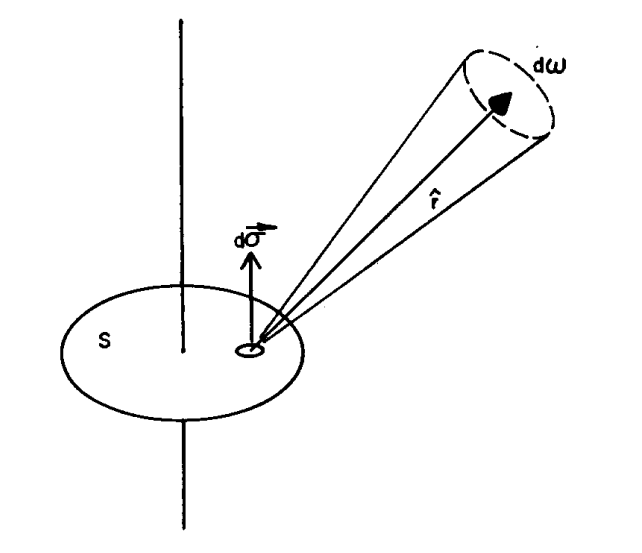
\includegraphics[width=.35\linewidth]{solidangle}
	\caption{Geometrical representation of a single plane detector \cite{Sullivan}.}
	\label{fig:planedetector}
\end{figure}
When performing a Monte Carlo simulation, the number of particles produced is large enough to consider one single particle as an infinitesimal $dN$, which is proportional to $dC=dGI$. It follows that
\begin{equation}\label{eq:dn}
dN \propto d\omega \cos\theta F(\omega)
\end{equation}
where $d\omega=d\varphi d\theta \sin\theta$, therefore from \eqref{eq:angD} and \eqref{eq:dn}, we have
\begin{equation}\label{eq:thetaMC}
dN \propto \cos^3\theta\sin\theta.
\end{equation}
Since $F$ does not depend on the azimuth angle, $\varphi$ is distributed according to a uniform distribution.

\subsection{Simulation procedure}

Muons crossing the scintillators can be generated starting from a \emph{seed event}, i.e. the coordinates $(x_0,y_0)$ of the muon impact point on the first scintillator surface and the angles $(\theta , \varphi)$ which define the muon direction.		
Impact point coordinates are uniformly generated $x \in [0,l]$ and $y \in [0,L]$, where $l = \SI{30}{cm}$ and $L = \SI{80}{cm}$ are the linear dimensions of the aligned scintillators.
The polar angle $\varphi$ is uniformly distributed in the range $\left[0,2\pi\right]$, whereas the zenith angle $\theta$ is generated in the range $\left[0,\pi/2\right]$ (i.e. the upper hemisphere) according to \eqref{eq:thetaMC}, by means of the \emph{try and catch} method.\\

The muons impact coordinates on the lower scintillator ($x^{'},y^{'}$) are computed from the seed event $\{x_0, y_0, \theta, \varphi \}$ according to

\begin{equation}
\begin{cases}
x^{'} = x_0 + r^{'} \sin \theta \cos \varphi   \\
y^{'} = y_0 + r^{'} \sin \theta \sin \varphi 
\end{cases}
\end{equation}

\noindent with
\begin{equation}
r^{'}= \frac{d}{\cos \theta}
\end{equation}
where $d$ is the distance between the upper scintillator (SC1) and the lower one (SC3)\footnote{Both in Section \ref{sec:geometric factor} calculations and in the Monte Carlo simulation, we have considered thick-less detectors. In the actual situation, with same dimensions aligned scintillators, a particle in the field of view of the telescope crosses the lower surface of the upper detector and the upper area of the lower one. Thus, $d$ will have to be measured according to this prescription.}.\\

The coincidence counts $N_{coinc}$ are given by events with $x^{'} \in [0,l]$ and $y^{'} \in [0,L]$, then we obtain the ratio of the number of muons which cross all the detectors to the total one $N_{tot}$ incident on the upper scintillator,

\begin{equation}
 g = \frac{N_{coinc}}{N_{tot}}.
\end{equation}

\begin{figure}[!htp]
	\centering
	\begin{subfigure}{.5\linewidth}
		\centering
		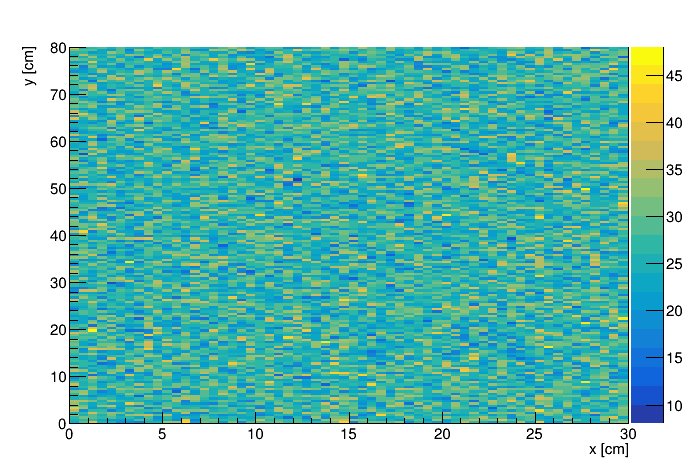
\includegraphics[width=\linewidth]{Scintillatore1}
		\caption{2D representation.}
	\end{subfigure}\hfill
	\begin{subfigure}{.5\linewidth}
		\centering
		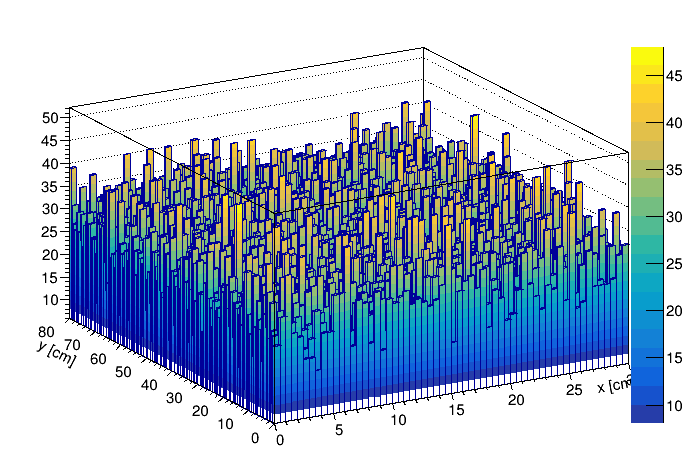
\includegraphics[width=\linewidth]{scintillatore13d}
		\caption{3D representation.}
	\end{subfigure}
	\caption{Generated muons distribution on the upper detector surface.}
	\label{fig:upper}	
\end{figure}
\begin{figure}[!htp]
	\centering
	\begin{subfigure}{.5\linewidth}
		\centering
		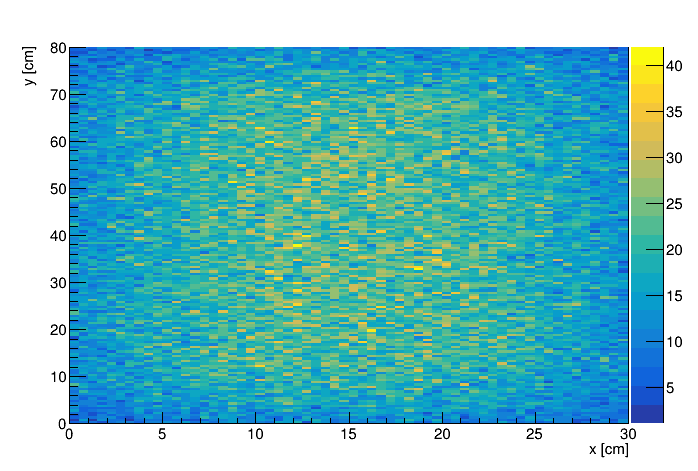
\includegraphics[width=\linewidth]{Scintillatore3}
		\caption{2D representation.}
	\end{subfigure}\hfill
	\begin{subfigure}{.5\linewidth}
		\centering
		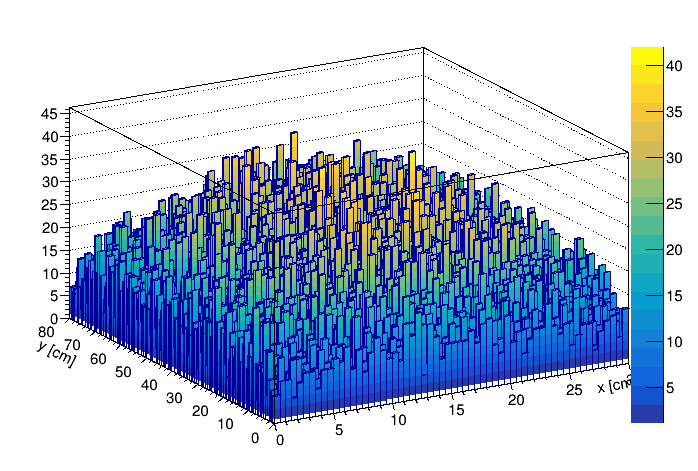
\includegraphics[width=\linewidth]{Scintillatore33d}
		\caption{3D representation.}
	\end{subfigure}
	\caption{Generated muons distribution on the lower detector surface.}
	\label{fig:lower}	
\end{figure}

The procedure is composed of $3500$ independent simulations and $250000$ muons have been generated in each of them. The spacial distributions of all generated muons on the surfaces of the upper and lower detectors are shown in Figure \ref{fig:upper} and \ref{fig:lower}. As expected, seed muons cover uniformly the surface of the upper scintillator, whereas the number of muons crossing the lower one show a decreasing trend at boundaries with respect to the internal area.
The distribution of the coefficient $g$, evaluated in each simulation, is fitted with a \emph{Gaussian}
\begin{equation}
\textrm{Gauss}(g;  \hat A , \hat g, \hat \sigma_{g})= \hat A e^{-\frac{(g -\hat g)^2}{2 {\hat \sigma_{g}}^2}}
\end{equation}
and the same procedure has been repeated twice: the first one refers to layouts displayed in Figure \ref{subfig:l1} and \ref{subfig:l2}, with an overall distance $d=\SI{8}{cm}$, whilst the second one refers to Figure \ref{subfig:l3} where $d=\SI{15}{cm}$. Fit results are shown in Figure \ref{fig:geom_eff}.

\begin{figure}[!htp]
	\centering
	\begin{subfigure}{.5\textwidth}
		\centering
		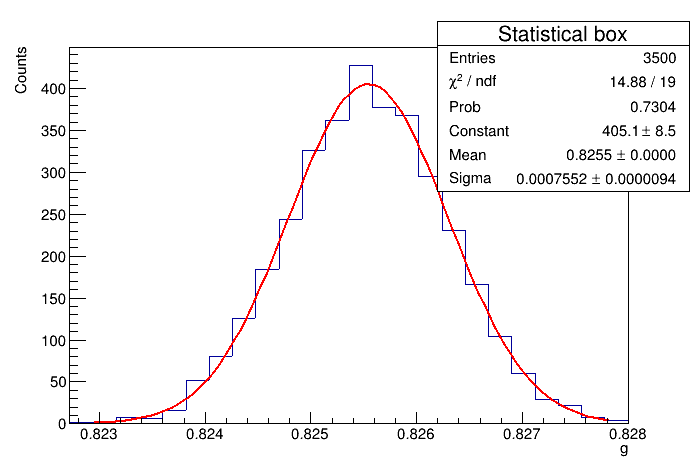
\includegraphics[width=\textwidth]{g_cerbero_up}
		\caption{Layout 1 and 2.}
	\end{subfigure}\hfill
	\begin{subfigure}{.5\textwidth}
		\centering
		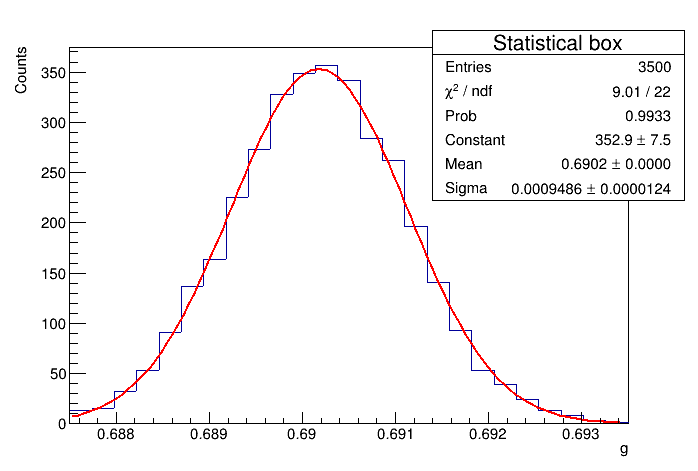
\includegraphics[width=\textwidth]{g_cerbero_middle}
		\caption{Layout 3.}
	\end{subfigure}
	\caption{Gaussian interpolation of the Monte Carlo results for the three layouts.}
	\label{fig:geom_eff}
\end{figure} 

\subsection{Comparison with analytical results}

Using $g$ we can rewrite Eq. \eqref{eq:intensity} as,
\begin{equation}\label{eq:g_Rozza}
	\begin{cases}
		I = C/\left(G_t \varepsilon_{t} \right)=S/\left(G_S \varepsilon_{s} \right)\\
		C = N_{double}/t \\
		S = N_{tot}/t
	\end{cases} \quad
	\Rightarrow\qquad \frac{C}{S} = \frac{N_{double}}{N_{tot}} \equiv g = \frac{G_t \varepsilon_{t}}{G_S \varepsilon_{s}}
\end{equation}
where $C$ and $S$ are the double and single counting rate respectively\footnote{For obvious reasons the time $t$ is the same in $C$ and $S$.}, $\varepsilon_{t}$ is the overall  efficiency of the particle telescope\footnote{See Section \ref{sec:geometric factor} for further details.} and $\varepsilon_{s}$ is the efficiency of the upper scintillator; $G_t$ and $G_S$ represent the geometric factor for the particle telescope and for the single detector, respectively. From the study made by Sullivan \cite{Sullivan} we know that the gathering power (i.e. the geometric factor) of a generic particle telescope is given by,
\begin{equation} \label{eq:gathering}
	\Gamma_F =\int_{\Omega}d\omega F(\omega)\int_{S}d\bm{\sigma}\cdot \mathbf{\hat{r}}
\end{equation}
where we remember that $F(\omega)$ represents the angular dependence of the radiation intensity. It follows that
\begin{equation}
	G_S = \int_{-X}^{X}\int_{-Y}^{Y}dxdy \int_{0}^{2\pi}d\phi \int_{0}^{1}\cos^3\theta d\left( \cos\theta\right) = 2\pi XY.
\end{equation}

Note that $X$ and $Y$ are half the length and width of the detector. Since all the scintillators have the same dimensions, we obtain $G_S = 0.3770\pm0.0006$ for all the detectors.\\
Finally, considering that $\varepsilon_{t} = \varepsilon_1 \varepsilon_3$ and $\varepsilon_{s} = \varepsilon_1$, we are able to estimate $g$, using the geometric factor of Eq. \eqref{eq:Thomas_simplified} and $G_S$ as reported below:
\begin{equation} \label{eq:G_MC}
	g = \frac{G_t\varepsilon_{t}}{G_S \varepsilon_{s}} = \frac{G_t \cdot \cancel \varepsilon_1\cdot \varepsilon_3}{G_S\cdot \cancel \varepsilon_1} = \frac{G_t}{G_S}\cdot \varepsilon_3
\end{equation}
Since the simulation procedure concern a purely geometrical effect, the efficiency of the detectors is assumed to be $1$ and \eqref{eq:G_MC} becomes
\begin{equation} \label{eq:G_MC_noeff}
	g = \frac{G_t}{G_S}
\end{equation}
hence, from \eqref{eq:G_MC_noeff} we can estimate $g$ and then compare it with the one obtained from the Monte Carlo. Results are reported in Table \ref{tab:G_t}.

\begin{table}[!htp]
	\centering
	\begin{tabular}{r|ccc}
		\toprule
		& $G_t/G_S$ & $\hat g$ & $p$-value\\
		\midrule
		Layout 1/2 & $0.825554\pm0.055870$ & $0.825544\pm0.000013$ & $0.9999$\\
		Layout 3 & $0.690180\pm0.051239$ & $0.690178\pm0.000016$ & $1.0000$\\
		\bottomrule
	\end{tabular}
	\caption{Accordance between $g=G_t/G_S$, given by the analytical calculation, and $\hat g$ estimated by means of the Monte Carlo method.}
	\label{tab:G_t}
\end{table}
In conclusion we can say the hypothesis made in the derivation of \eqref{eq:Thomas} in Section \ref{sec:geometric factor} are reasonable from the geometrical point of view due to the $p$-values largely above the adopted significance level equal to $0.05$.



\section{Uniformity studies}

\label{sec:uniformity_studies}

Subsequent to calculating the efficiency for each scintillator, a uniformity measurement of the latter is fundamental, in order to identify which portions of the detector work better or worse than the others. Further details will be explained in Section \ref{sec:uniformity}, nevertheless, the experimental layouts represented in Figure \ref{fig:uniformity} highlight the need to develop a Monte Carlo simulation.\\

In fact, when computing efficiency as
\begin{equation}
\varepsilon = \frac{N_{triple}}{N_{double}}
\end{equation}
\begin{figure}[!tbp]
	\centering
	\begin{subfigure}{.3\linewidth}
		\centering
		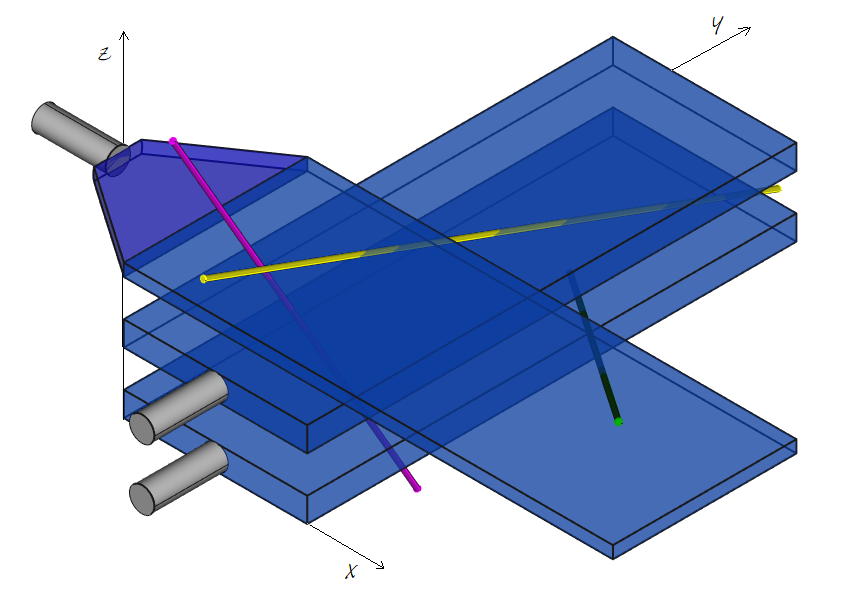
\includegraphics[width=\linewidth]{ParticlesMC}
		\caption{Axonometric projection.} 
		\label{subfig:particles}
	\end{subfigure}\hfill
	\begin{subfigure}{.3\linewidth}
		\centering
		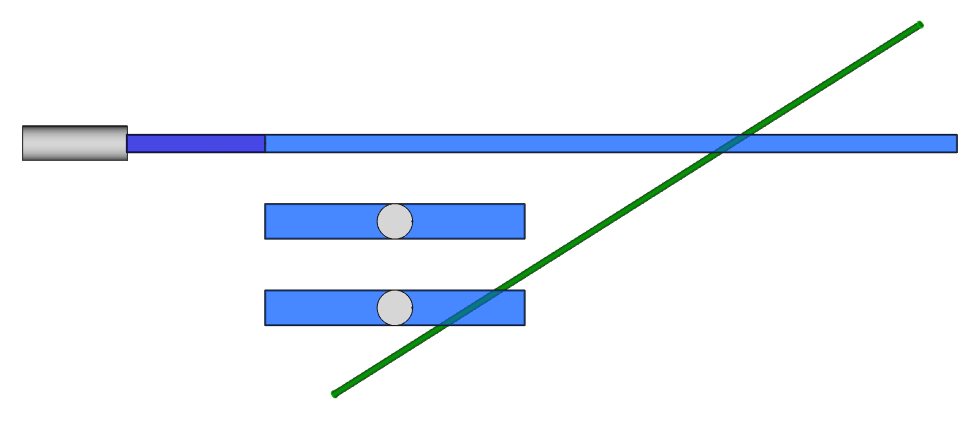
\includegraphics[width=\linewidth]{FalseDoppie_Lateral}
		\caption{Lateral view.} 
		\label{subfig:fd_lateral}
	\end{subfigure}\hfill
	\begin{subfigure}{.3\linewidth}
		\centering
		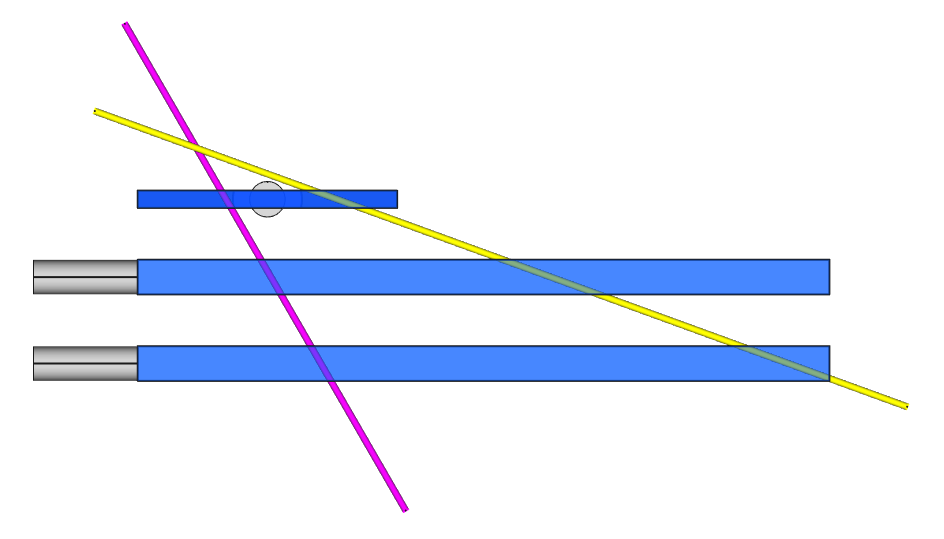
\includegraphics[width=\linewidth]{FalsaZona_Front}
		\caption{Front view.} 
		\label{subfig:fz_front}
	\end{subfigure}
	\caption{The purple particle is a true double, the yellow one contributes to a wrong area, whilst the green particle is a false double.} 
	\label{fig:uniformity_mc}
\end{figure}
the not-aligned geometry provides a systematic error that leads to an overestimate of $N_{double}$, thus an underestimated efficiency. The evidence of this behavior is clear from Figure \ref{fig:uniformity_mc}, where we can identify three event-types: $N_{double}^{t}$ as the true double counts (purple particle), $N_{double}^{wa}$ as the number of doubles referred to a wrong area (yellow particle) and $N_{double}^{f}$ as a false double count (since the middle-scintillator is not crossed by the green particle). With respect to the aligned geometry where the measured counts are $N_{double}=N_{double}^{t}$ and $N_{triple}=N_{triple}^{t}$, now
\begin{equation}\label{N_measured}
\left\{
\begin{array}{l}
N_{double}=N_{double}^{t}+N_{double}^{wa}+N_{double}^{f}\\\\
N_{triple}=N_{triple}^{t}+N_{triple}^{wa}
\end{array}
\right.
\end{equation}
therefore, if one define a \emph{wrong-area} efficiency\footnote{In $\varepsilon_{wa}$ formula \emph{double}/\emph{triple} subscripts have been omitted since the \emph{wrong-area} effect is purely geometric, thus it works both for \emph{triple} and \emph{double} counts in the same way.} as
\begin{equation}\label{eff_wa}
\varepsilon_{wa} = \frac{N^t}{N^t+N^{wa}}
\end{equation}
and a \emph{geometrical} efficiency as
\begin{equation}\label{eff_geom}
\varepsilon_{g} = \frac{N^t+N^{wa}}{N^t+N^{wa}+N^f}
\end{equation}
it is clear that from $N_{triple}^t=\varepsilon\cdot N_{double}^t$, \eqref{N_measured}, \eqref{eff_wa} and \eqref{eff_geom} follows that
\begin{equation}
\varepsilon_{wa}\cdot N_{triple} = \varepsilon\cdot\varepsilon_{wa}\cdot\varepsilon_g\cdot N_{double}
\end{equation}
thus, the efficiency $\varepsilon$ of the middle-scintillator (due to radiation-matter interaction) is given by
\begin{equation}\label{eq:eff_correct}
\varepsilon = \frac{N_{triple}}{\varepsilon_g\cdot N_{double}}
\end{equation}
The main purpose of the following Monte Carlo procedure is the simulation of the explained geometrical effect and an estimation of the weight defined in \eqref{eff_geom}, needed as a correction on the measured double counts.

\subsection{Simulation procedure}
The implemented solution is based on the generation of $M$ muons in the volume of the upper detector, i.e. we have four uniformly distributed random numbers $x_1\in\left[0, L\right]$, $y_1\in\left[0, l\right]$, $z_1\in\left[z_1^{d},z_1^{u}\right]$ and $\varphi\in\left[0, 2\pi\right]$, where $L$, $l$ are the scintillators length and width, respectively, $z_1^{d/u}$ are the $z$-coordinates of the lower/upper surface of the detector and $\varphi$ is the azimutal angle. Finally the zenith angle $\theta\in\left[0, \pi/2\right]$ is generated following \eqref{eq:thetaMC} distribution by means of what is known as \emph{try and catch} method. Since we deal with MIPs, one can reasonably neglect their deflection (following interaction with detectors) and describe their trajectory by making use of straight line equations
\begin{equation}\label{eq:straight}
\left\{
\begin{array}{l}
x = x_1 + t\cdot\sin\theta\cos\varphi\\\\
y = y_1 + t\cdot\sin\theta\sin\varphi\\\\
z = z_1 + t\cdot\cos\theta
\end{array}
\right.
\end{equation}
From \eqref{eq:straight} it follows that
\begin{equation}
\left\{
\begin{array}{l}
x = \textrm{fixed}\\\\
y = y_1 + (x-x_1)\cdot\tan\varphi\\\\
z = z_1 + (x-x_1)\cdot\displaystyle\frac{1}{\tan\theta\cos\varphi}
\end{array}
\right.
\end{equation}
then
\begin{equation}
\left\{
\begin{array}{l}
x = x_1 + (y-y_1)\cdot\displaystyle\frac{1}{\tan\varphi}\\\\
y = \textrm{fixed}\\\\
z = z_1 + (y-y_1)\cdot\displaystyle\frac{1}{\tan\theta\sin\varphi}
\end{array}
\right.
\end{equation}
and
\begin{equation}
\left\{
\begin{array}{l}
x = x_1 + (z-z_1)\cdot\tan\theta\cos\varphi\\\\
y = y_1 + (z-z_1)\cdot\tan\theta\sin\varphi\\\\
z = \textrm{fixed}
\end{array}
\right.
\end{equation}

Due to non-negligible scintillators height, the simulation procedure recognizes that a muon crosses the middle detector\footnote{The case of particles crossing the middle scintillator without passing through its surfaces is excluded by the simulation, since of course they could not cross the lower detector, which is aligned with the middle one.} if it passes through the lower or upper surface. Instead, concerning the lower detector, it can be crossed by a particle even in the lateral areas without involving upper or lower surfaces.\\

Now we can define a boolean variable $sc_i$ which is \emph{true} if the particle crosses the $i$-scintillator, otherwise it is \emph{false}, and two additional variables $sc_2^a$ and $sc_2^{wa}$ which are referred to the correct and wrong area of the middle detector, respectively. As a consequence, events are classified in the following way:
\begin{equation}
\begin{array}{l}
sc_1 \,\wedge\, sc_2^a \,\wedge\, sc_3 \qquad \Rightarrow \qquad N_{double}^t\\\\
sc_1 \,\wedge\, sc_2^{wa} \,\wedge\, sc_3 \qquad \Rightarrow \qquad N_{double}^{wa}\\\\
sc_1 \,\wedge\, \textrm{\texttt{not}} \left(sc_2^a \vee sc_2^{wa}\right) \,\wedge\, sc_3 \qquad \Rightarrow \qquad N_{double}^f
\end{array}
\end{equation}
hence, the geometrical efficiency is calculated according to \eqref{eff_geom}. The described procedure is repeated $N_{MC}$ times, in order to reduce the statistical error, and an histogram of $\varepsilon_{g}$ is produced. The details of the developed \texttt{C++} functions are reported in Appendix \ref{app:eff_geom_MC}.\\

\begin{table}[!hbp]
	\centering
	\begin{tabular}{cc}
	\toprule
	Variable & Value ($\si{\centi\meter}$)\\
	\midrule
	$L$ & $80.0$\\
	$l$ & $30.0$\\
	$h_1$ & $1.0$\\
	$h_2$ & $3.8$\\
	$h_3$ & $3.8$\\
	$d_1$ & $2.5$\\
	$d_2$ & $2.0$\\
	\bottomrule
	&\\
	\multicolumn{2}{c}{\footnotesize (a) \emph{Caronte - Minosse}}
	\end{tabular}\qquad\qquad
	\begin{tabular}{cc}
		\toprule
		Variable & Value ($\si{\centi\meter}$)\\
		\midrule
		$L$ & $80.0$\\
		$l$ & $30.0$\\
		$h_1$ & $3.8$\\
		$h_2$ & $1.0$\\
		$h_3$ & $3.8$\\
		$d_1$ & $7.0$\\
		$d_2$ & $7.0$\\
		\bottomrule
		&\\
		\multicolumn{2}{c}{\footnotesize (b) \emph{Cerbero}}
	\end{tabular}
	\caption{Geometrical parameters of the detectors setup. $h_{1/2/3}$ represents the height of the upper/middle/lower scintillator, while $d_1$, $d_2$ are the distances between the upper and the middle detector and between the middle and the lower one, respectively.} \label{tab:length}
\end{table}

Each length parameter has been measured by means of a meter-stick: measurements are summed up in Table \ref{tab:length}.
\begin{figure}[!htp]
	\centering
	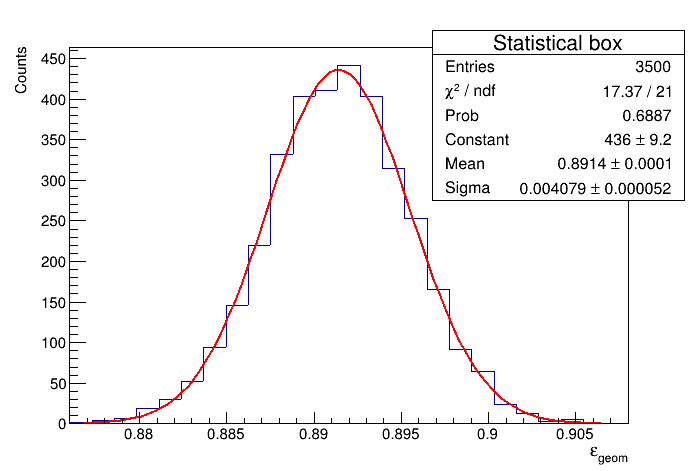
\includegraphics[width=.7\linewidth]{eff_geom_MC}
	\caption{Geometrical efficiency distribution.} 
	\label{fig:mc_eff_g}
\end{figure}
Figure \ref{fig:mc_eff_g} shows a resulting histogram referred to \emph{Caronte - Minosse} layout 3, with $M=250000$ and $N_{MC}=3500$, fitted with a \emph{Gaussian} distribution\footnote{With respect to the statistical box of Figure \ref{fig:mc_eff_g}, calling Constant $=C$, Mean $=\langle\varepsilon_{g}\rangle$ and Sigma $=\sigma$, the Gaussian distribution is $G(\varepsilon_{g})=C\cdot \exp\left(- \left(\varepsilon_{g}- \langle\varepsilon_{g}\rangle\right)^2/\left(2\sigma^2\right)\right)$.}, as expected by considering the \emph{central limit theorem}. The correspondence between simulated efficiencies and the Gaussian fit-function is clear, since
\begin{equation}
P_{21}\left(\chi^2 \geq \chi^2_{obs} \right) = 68.87\,\%
\end{equation}
where $21$ is the number of degrees of freedom and $\chi^2_{obs}$ is the observed $\chi^2$-value.\\

Finally, simulated geometrical efficiencies for each layout (with respect to Figure \ref{fig:uniformity}) are summed up in Table \ref{tab:all-effg}.

\begin{table}[!hbp]
	\centering
	\begin{tabular}{r|cc}
	\toprule
	&\emph{Caronte - Minosse} & \emph{Cerbero}\\
	\midrule
	Layout 1 & $0.939748$ & $0.905542$\\
	Layout 2 & $0.938381$ & $0.903697$\\ 
	Layout 3 & $0.891402$ & $0.850164$\\
	\bottomrule
	\end{tabular}
	\caption{Simulated geometrical efficiencies.}\label{tab:all-effg}
\end{table}

\subsection{Uncertainty estimation}

As discussed above, the main purpose of this Monte Carlo simulation is to estimate $\varepsilon_{g}$ which leads to the rejection of geometrical systematic error, but the procedure itself is affected by an error we want to keep track of.\\

A source of error on $\varepsilon_{g}$ is given by the uncertainty on the measured geometrical parameters $\pi_j$ that enter in the simulation, thus the geometrical efficiency is estimated several times by varying these parameters in the range $\left[\pi_j-\sigma_{\pi_{j}}, \pi_j+\sigma_{\pi_{j}} \right]$. Therefore, the uncertainty on $\varepsilon_{g}$ is empirically determined as the maximum deviation from the mean efficiency $\langle\varepsilon_{g}\rangle$.\\
\begin{equation}
\sigma_{\varepsilon_{g}}=\max_k\left|\varepsilon_{g_k}  -\langle\varepsilon_{g}\rangle\right|
\end{equation}
where $k=1, ..., 3^J$ and $J$ is the number of parameters $\pi_j$.\\

The computational cost of this method grows exponentially, for this reason it is worth restricting the analysis only on variables affected by the higher uncertainties. $L,l, h_i$ are given by the manufacturer, hence the most relevant errors are on the distances $d_1$ and $d_2$ between detectors: $\sigma_d=\SI{0.5}{cm}$ is assumed for both $d_1$ and $d_2$ as a reasonable upper limit, in order to evaluate the impact of a change of their central values on the estimated $\varepsilon_{g}$. Table \ref{tab:err-effg} shows the results.

\begin{table}[!hbp]
	\centering
	\begin{tabular}{r|cc}
		\toprule
		&\emph{Caronte - Minosse} & \emph{Cerbero}\\
		\midrule
		Layout 1  & $0.940\pm 0.005$ & $0.906\pm 0.005$\\
		Layout 2 & $0.938\pm 0.005$ & $0.904\pm 0.005$\\ 
		Layout 3 & $0.892\pm 0.009$ & $0.850\pm 0.008$\\
		\bottomrule
	\end{tabular}
	\caption{Simulated geometrical efficiencies, errors estimation included.}\label{tab:err-effg}
\end{table}

